\textbf{\uline{Exemplo 02:}}

	\begin{center}
		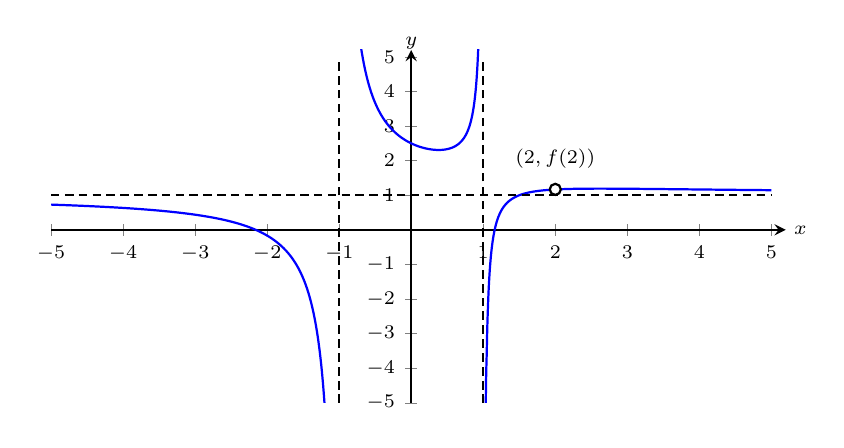
\begin{tikzpicture}[font=\scriptsize]
			\begin{axis}[thick,smooth,axis lines=middle,width=0.9\textwidth,
				height=0.5\textwidth,
				xmin=-5,xmax=5.2,ymin=-5,ymax=5.2,
				every axis x label/.style={
					at={(ticklabel* cs:1.02)}},
				every axis y label/.style={
					at={(ticklabel* cs:1.02)}},
				xlabel=$x$,ylabel=$y$,ytick distance=1,samples=200,smooth]
				\addplot[blue,domain=-5:-1.01] {(x-1.5)/(x^2-1) + 1};
				\addplot[blue,domain=-0.99:0.99] {(x-1.5)/(x^2-1) + 1};
				\addplot[blue,domain=1.01:5] {(x-1.5)/(x^2-1) + 1};
				\addplot[densely dashed,domain=-5:5] ({1},{x});
				\addplot[densely dashed,domain=-5:5] ({-1},{x});
				\addplot[densely dashed,domain=-5:5] {1};
				\addplot[mark=*,mark size=2pt,fill=white] coordinates {(2,1.17)};
				\node[label={90:{$(2,f(2))$}}] at (axis cs:2,1.17) {};
			\end{axis}
		\end{tikzpicture}
	\end{center}